\documentclass[12pt,oneside,reqno]{amsart}

\addtolength{\hoffset}{-2.25cm}
\addtolength{\textwidth}{4.5cm}
\addtolength{\voffset}{-2.5cm}
\addtolength{\textheight}{5cm}
\setlength{\parskip}{0pt}
\setlength{\parindent}{15pt}

\usepackage{amsthm}
\usepackage{amsmath}
\usepackage{amssymb}
\usepackage[colorlinks = true, linkcolor = black, citecolor = black, final]{hyperref}

\usepackage{graphicx}
\usepackage{multicol}
\usepackage{ marvosym }
\usepackage{wasysym}
\usepackage{tikz}
\usepackage[utf8]{inputenc}
\usepackage{multirow}
\usepackage{xcolor}

\usepackage{caption}
\captionsetup[table]{skip=10pt}

\newcommand{\ds}{\displaystyle}
\DeclareMathOperator{\sech}{sech}


\setlength{\parindent}{0in}

\pagestyle{empty}

\usepackage{color}
\begin{document}


{\scshape IIT,Kanpur} \hfill  \hfill {\scshape  CS610 (2020-2021)}
 \thispagestyle{empty}

\smallskip

\hrule
\bigskip

    \begin{center}
		\begin{LARGE}
	      Assignment 2\\[5pt]
		\end{LARGE}
	Aditya Jain (20111004) $\mid$ Mahi Agrawal (20111029)\\

\texttt{adityaj20@iitk.ac.in | maahi20@iitk.ac.in}\\Group Id: 23

	\end{center}

  \bigskip

\begin{LARGE}
		\textbf{Part 1}
	\end{LARGE}

 \begin{table}[h]
     \centering
     \begin{tabular}{|c|c|}
        \hline
        Program     &  Total Machine Access\\
        \hline
        \hline
         prog1:&  140525433   \\
         prog2:& 2718547\\
         prog3:& 10621695\\
         prog4:& 1064755\\

\hline
     \end{tabular}
     \caption{Total Machine Access}
     \label{tab:Total Machine Access}
 \end{table}
 \textbf{Note: Total Machine Accesses will differ from one run to another, these won't be exactly same.}\\\\

\begin{LARGE}
		\textbf{\\Part 2\\ }
	\end{LARGE}
Graphs for prog1, prog2, prog3, and prog4 are as follows:\\
	\begin{figure}[h]
    \centering
		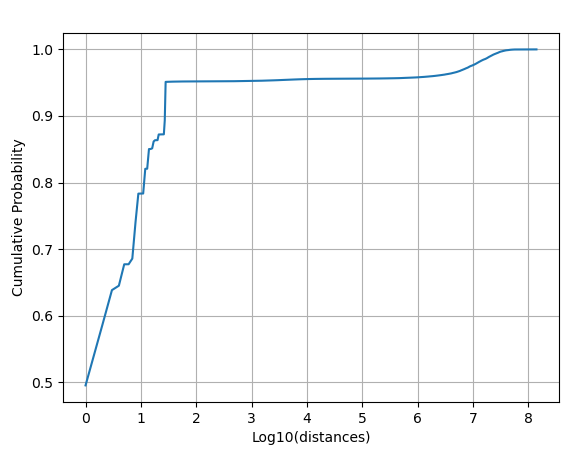
\includegraphics[scale=1]{q2_prog1.png}
    	\caption{prog1}
\end{figure}
\newpage
\begin{figure}[h]
    \centering
		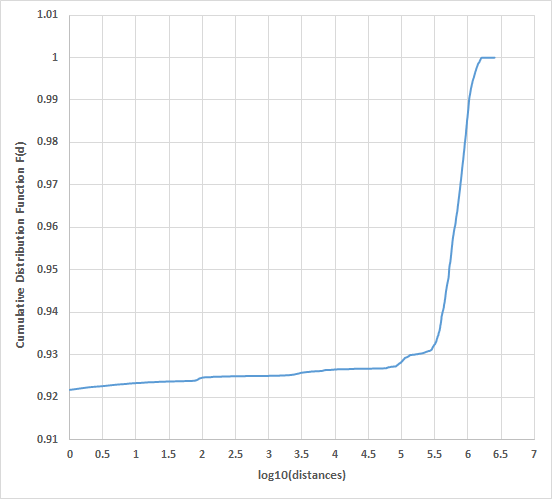
\includegraphics[scale=1.1]{q2_prog2.png}
    	\caption{prog2}
\end{figure}

\bigskip
\begin{figure}[h]
    \centering
		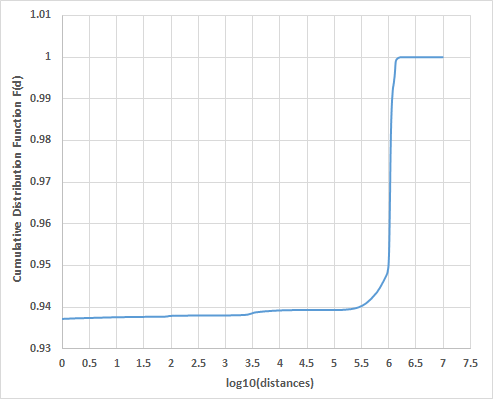
\includegraphics[scale=1.2]{q2_prog3.png}
    	\caption{prog3}
\end{figure}
\newpage

\bigskip
\begin{figure}[h]
    \centering
		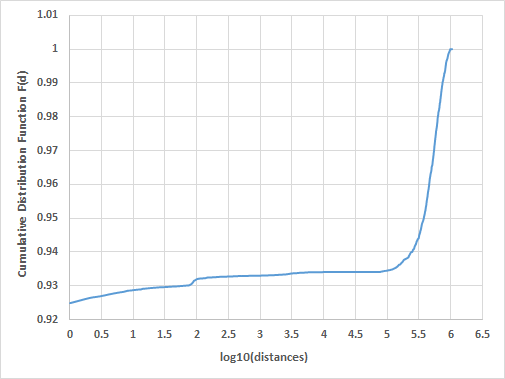
\includegraphics[scale=1.2]{q2_prog4.png}
    	\caption{prog4}
\end{figure}

\bigskip
By the above-given graphs, we can say that 92\% - 93\% of blocks enjoy access distances of 1 in prog2, prog3 and prog4. It essentially means that a block is consecutively accessed one or more times and implies that there is a high chance of them enjoying locality of reference, i.e. a large number of cache hits. Still, these can only be confirmed when we use a cache to do the same analysis. \\\\

We can also not say that the program will enjoy a good locality of reference as for the case where block requests are as follows: 2,2,3,3,4,4,5,5,10,17,17... In this, the blocks have access distance as one, but still, the number of cache hits will only be 50\% which is not good enough.\\

In prog1 approximately 95\% of blocks have access distance of equal or smaller than 20, so in-fact prog1 might enjoy a good locality of reference and a large number of cache hits, which is again verified in part 3, but the prog1 will have lesser locality as compared to other 3 programs.\\

As the prog1 has the knee around log(1.3), which means the access distance is approximately 20, and F(20) $\approx$ 95\% hence the fully associative cache with the crude upper bound of \textbf{20*64 = 1280 byte $\approx$ 2048 byte cache} should be able to capture all the reuses for all the four programs\\

\textbf{Note :-} For finding crude upper bound we have considered prog1 as the prog1 has the 0.95 at the greater access distance as compared to other programs.

\newpage
\begin{LARGE}
		\textbf{\\Part 3\\ }
\end{LARGE}
\begin{table}[h]
\centering
\caption{Number of Cache Hits and Misses}
\begin{tabular}{|l|r|r|r|r|}

\hline
 & \multicolumn{1}{c|}{prog1} & \multicolumn{1}{c|}{prog2} & \multicolumn{1}{c|}{prog3} & \multicolumn{1}{c|}{prog4} \\ \hline
Total Accesses & 140525433 & 25,18,630 & 97,90,965 & 10,64,726 \\
Cache Hits     & 133733928 & 22,81,363 & 91,35,892 & 9,34,364  \\
Cache Misses   & 6791505   & 2,37,267  & 6,55,073  & 1,30,362  \\
\hline
Hit Rate       & 95.17\%   & 90.58\%   & 93.31\%   & 87.76\%  \\
\hline
\end{tabular}
\end{table}

\bigskip
Graphs of prog1, prog2, prog3 and prog4 after adding cache in the system are as follows:
\begin{figure}[h]
    \centering
		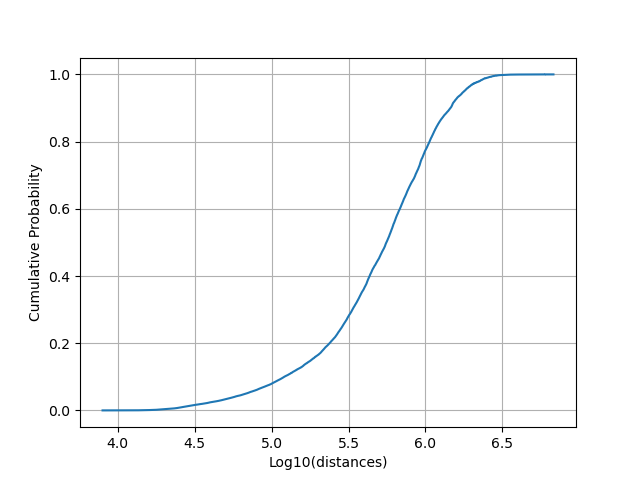
\includegraphics[scale=0.7]{q3_prog1.png}
    	\caption{prog1}

\end{figure}\\

\newpage
	\begin{figure}[h]
    \centering
		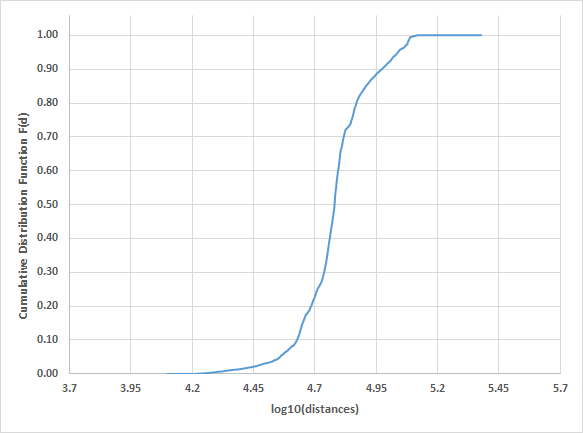
\includegraphics[scale=1.1]{q3_prog2.png}
    	\caption{prog2}
    	\end{figure}

\bigskip
    \begin{figure}[h]
    \centering
		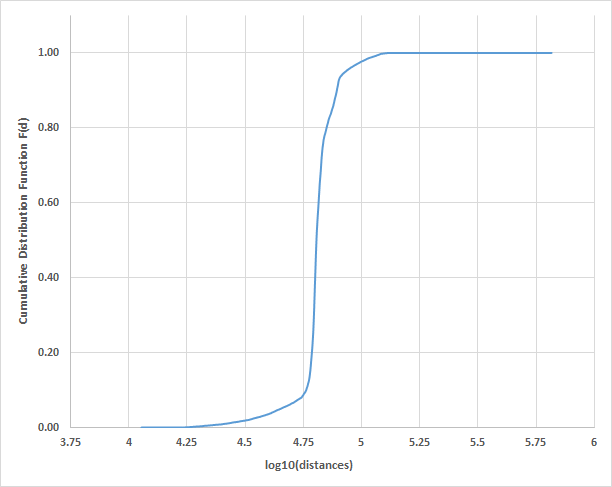
\includegraphics[scale=1.1]{q3_prog3.png}
    	\caption{prog3}
    	\end{figure}


 \newpage
  \begin{figure}[h]
\centering
	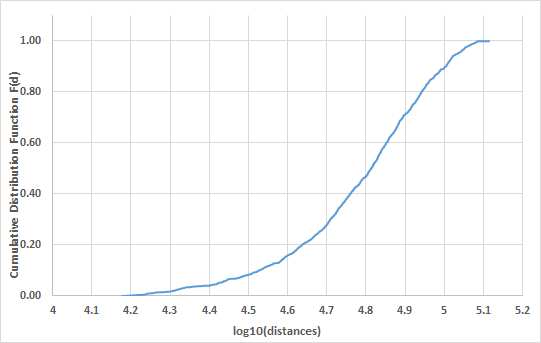
\includegraphics[scale=1.1]{q3_prog4.png}
	\caption{prog4}
	\end{figure}

\textbf{Note: F(d) represents the number access smaller than or equal to d divided by total number of access distance }\\

\textbf{The curves before and after the cache vary} The reason for this is as follows:-\\

\textbf{We observed in part 2 that the} large number of blocks have access distance equals to 1 for prog2, prog3,prog4 and lesser than or equal to 20 for prog1.\\

\textbf{In this part we observed that} the F(d) before 4.5 (or access distance 31622) is approximately zero (0). This is because access distance of majority of access is equals to 1,(for prog2 , prog3 and prog4) and less than or equal to 20(for prog1) and all these accesses hit in cache.\\


    If we observe the above two points we can say that the programs enjoy locality of reference \texttt{i.e spatial locality and temporal locality} for the large number of accesses due to the smaller access distance which we observed in part 2. This essentially means that large number of accesses hits in the cache and hence do not turn up in the miss trace and hence we can observe F(d) approximately equals to zero before 4.5.\\


\textbf{This can also be verified by the Table 2, which shows that hit rate for programs are high ($\approx$ 87\% - 95\%)}\\


 There is a spike in the curve at the log(access distance) $\approx$ 4.5, which correspond to the access distance of \textbf{31622}, which approximately equals to the number of blocks in cache \texttt{i.e 32768}, this signifies that the large number of cache misses are \textbf{ capacity misses.}






\newpage
\begin{LARGE}
		\textbf{\\Part 4  }
	\end{LARGE}

\begin{table}[h]

\begin{tabular}{llllllll}
\\
\hline
\multicolumn{1}{|c|}{\multirow{2}{*}{\textbf{Blocks Shared by}}} &
  \multicolumn{4}{c|}{\textbf{Programs}} \\
   \cline{2-5}
\multicolumn{1}{|c|}{} &
  \multicolumn{1}{c|}{Prog1} &
  \multicolumn{1}{c|}{Prog2} &
  \multicolumn{1}{c|}{Prog3} &
  \multicolumn{1}{c|}{Prog4} \\
  \hline
\multicolumn{1}{|c|}{Private} &
  \multicolumn{1}{c|}{432} &
  \multicolumn{1}{c|}{432} &
  \multicolumn{1}{c|}{441} &
  \multicolumn{1}{c|}{8621}  \\
\multicolumn{1}{|c|}{Two Threads} &
  \multicolumn{1}{c|}{70} &
  \multicolumn{1}{c|}{8262} &
  \multicolumn{1}{c|}{63} &
  \multicolumn{1}{c|}{57410}  \\
\multicolumn{1}{|c|}{Three Threads} &
  \multicolumn{1}{c|}{1872} &
  \multicolumn{1}{c|}{16384} &
  \multicolumn{1}{c|}{0} &
  \multicolumn{1}{c|}{6} \\
\multicolumn{1}{|c|}{Four Threads} &
  \multicolumn{1}{c|}{32456} &
  \multicolumn{1}{c|}{40958} &
  \multicolumn{1}{c|}{1} &
  \multicolumn{1}{c|}{0}  \\
\multicolumn{1}{|c|}{Five Threads} &
  \multicolumn{1}{c|}{143251} &
  \multicolumn{1}{c|}{5} &
  \multicolumn{1}{c|}{1} &
  \multicolumn{1}{c|}{0} \\
\multicolumn{1}{|c|}{Six Threads} &
  \multicolumn{1}{c|}{244970} &
  \multicolumn{1}{c|}{0} &
  \multicolumn{1}{c|}{0} &
  \multicolumn{1}{c|}{0}  \\
  \multicolumn{1}{|c|}{Seven Threads} &
  \multicolumn{1}{c|}{173832} &
  \multicolumn{1}{c|}{1} &
  \multicolumn{1}{c|}{1} &
  \multicolumn{1}{c|}{2}   \\
  \multicolumn{1}{|c|}{Eight Threads} &
  \multicolumn{1}{c|}{124528} &
  \multicolumn{1}{c|}{11} &
  \multicolumn{1}{c|}{65546} &
  \multicolumn{1}{c|}{12}  \\
  \hline
  \multicolumn{1}{|c|}{Total} &
  \multicolumn{1}{c|}{721411} &
  \multicolumn{1}{c|}{66053} &
  \multicolumn{1}{c|}{66053} &
  \multicolumn{1}{c|}{66051}\\
  \hline
\end{tabular}
 \caption{Sharing Profile}
\end{table}
 \smallskip
By looking at sharing profile we can say that the number of local or the private blocks used by each thread are very less, and number of shared blocks are high. The number of private blocks are almost same for prog1, prog2 and prog3,  whereas for prog4 the number of private blocks are comparatively higher. This shows that prog4's execution involves large number of local variables relatively to other programs, moreover most of the blocks are shared by two threads in prog4. \\

In prog1, a large number of blocks are shared between five, six and seven, and eight threads. It shows that prog1's execution involves a large amount of shared data.



\end{document}
